\begin{tikzpicture}[<->,>=stealth',shorten >=0.1pt,auto,
  thick,main node/.style={circle,fill=blue!20,draw,font=\sffamily\Large\bfseries}]


\node (fig1) at (-3,-5)
       {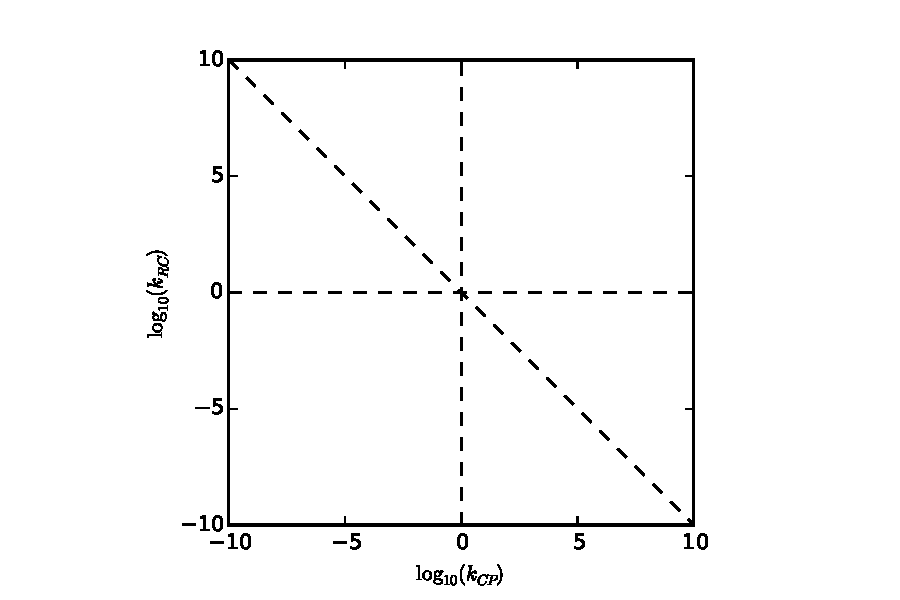
\includegraphics[scale=0.8]{C:/Users/Carlos/Documents/Tesis-IGP/code/Theory/ZonesSR.pdf}};

\node[circle,fill= blue!20,draw, minimum size=0.6cm,inner sep= 0] (R) at (-5.5,-4.5){R};
\node[circle,fill=blue!20,draw,minimum size=0.3cm, inner sep = 0] (C) at (-4.5,-3.8) {C};
\node[circle,fill=blue!20,draw,minimum size=1.cm,inner sep = 0](P) at (-5.5,-3.) {P};

 \path[every node/.style={font=\sffamily\small}]

(R) edge [<-,red] (C)
(R) edge [<-,red] (P)
(P) edge [->,red] (C);


\node[circle,fill= blue!20,draw, minimum size=0.3cm,inner sep= 0] (R) at (-4.5,-7.8){R};
\node[circle,fill=blue!20,draw,minimum size=0.6cm, inner sep = 0] (C) at (-3.5,-6.7) {C};
\node[circle,fill=blue!20,draw,minimum size=1.cm,inner sep = 0](P) at (-4.5,-5.6) {P};

 \path[every node/.style={font=\sffamily\small}]

(R) edge [<-,red] (C)
(R) edge [<-,red] (P)
(P) edge [->,red] (C);


\node[circle,fill= blue!20,draw, minimum size=1.cm,inner sep= 0] (R) at (-3.4,-3.6){R};
\node[circle,fill=blue!20,draw,minimum size=0.3cm, inner sep = 0] (C) at (-4.3,-2.6) {C};
\node[circle,fill=blue!20,draw,minimum size=0.6cm,inner sep = 0](P) at (-3.4,-2.1) {P};

 \path[every node/.style={font=\sffamily\small}]

(R) edge [<-,red] (C)
(R) edge [<-,red] (P)
(P) edge [->,red] (C);



\node[circle,fill= blue!20,draw, minimum size=1.cm,inner sep= 0] (R) at (-1.5,-4.1){R};
\node[circle,fill=blue!20,draw,minimum size=0.6cm, inner sep = 0] (C) at (-0.3,-3) {C};
\node[circle,fill=blue!20,draw,minimum size=0.3cm,inner sep = 0](P) at (-1.5,-2.1) {P};

 \path[every node/.style={font=\sffamily\small}]

(R) edge [<-,red] (C)
(R) edge [<-,red] (P)
(P) edge [->,red] (C);


\node[circle,fill= blue!20,draw, minimum size=0.6cm,inner sep= 0] (R) at (-0.1,-7){R};
\node[circle,fill=blue!20,draw,minimum size=1.0cm, inner sep = 0] (C) at (-1,-5.9) {C};
\node[circle,fill=blue!20,draw,minimum size=0.3cm,inner sep = 0](P) at (-0.1,-5.2) {P};

 \path[every node/.style={font=\sffamily\small}]

(R) edge [<-,red] (C)
(R) edge [<-,red] (P)
(P) edge [->,red] (C);


\node[circle,fill= blue!20,draw, minimum size=0.3cm,inner sep= 0] (R) at (-2.55,-7.8){R};
\node[circle,fill=blue!20,draw,minimum size=1.cm, inner sep = 0] (C) at (-1.8,-6.7) {C};
\node[circle,fill=blue!20,draw,minimum size=0.6cm,inner sep = 0](P) at (-2.55,-5.7) {P};

 \path[every node/.style={font=\sffamily\small}]

(R) edge [<-,red] (C)
(R) edge [<-,red] (P)
(P) edge [->,red] (C);


   
\end{tikzpicture}
